Для работы с репозиторием сначала нужно зарегестрироваться на GitHub, перейдя по ссылке: : https://github.com/ и заполнить всю необходимую информацию о себе [6].

Затем переходим по ссылке: https://github.com/nickkolok/chas-ege/. Далее нажимаем на зелёную кнопку с надписью «Code», и копируем ссылку репозитория. Лучше сделать это сразу, потому что Ubuntu на VirtualBox может сильно нагружать компьютер, и открыть вкладку с браузером может быть проблематично из-за нагрузки. (Если возникли проблемы с копирование ссылки, то можно открыть браузер внутри Ubuntu, перейти по ссылке и скопировать ссылку репозитория в нём.)

\begin{figure}[h]
		\centering
		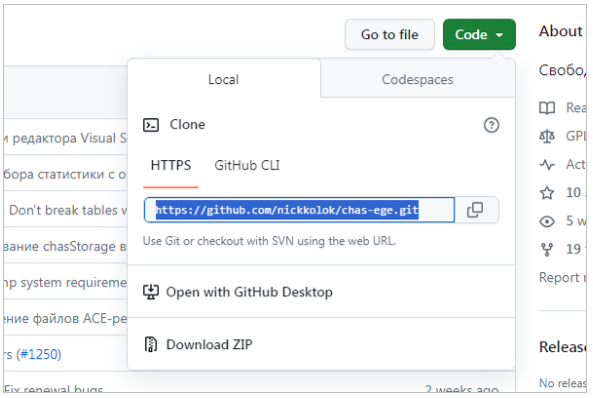
\includegraphics[width=0.9\linewidth]{VM/6.png}
\caption{Github. Ссылка на репозиторий.}
\label{ris:image}
\end{figure}

• Далее снова заходим в терминал и создаём папку на рабочем столе командой: mkdir <название папки>. Можно убедиться, что папка создана, с помощью команды: ls. Мы увидим все папки на рабочем столе, среди которых должна быть только что созданная.Затем заходим в папку командой: cd <название папки>, и клонируем себе репозиторий командой: git clone <ссылка на репозиторий >

• Добавляем себе ссылку на основной репозиторий проекта с помощью команды: git remote add upstream <ссылка на репозиторий> и убеждаемся, что он подключился, командой: git fetch upstream 

• Собираем проект командой: grunt. Важно выполнять эту команду в папке, в которую мы и склонировали репозиторий.

• Открываем файл dist/sh/otladka.html в браузере командой: «open otladka.html», и запускаем любой шаблон, для проверки, в открывшемся окне.


\begin{figure}[h]
		\centering
		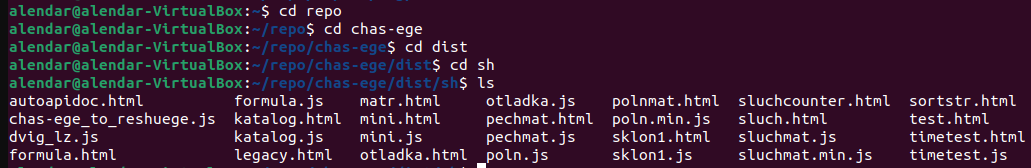
\includegraphics[width=1\linewidth]{VM/7.png}
\caption{Путь к файлу otladka.html.}
\label{ris:image}
\end{figure}